\chapter{\textit{Shift Graphs}}
\label{cap:shift}

\begin{definicao}
Um \textit{shift graph} de parâmetro $n$, denotado $S_n$, é um grafo cujos vértices são os pares ordenados $(a,b)$, onde $1 \leq a < b \leq n$, e dois vértices $(a,b)$ e $(c,d)$ são adjacentes se $b = c$ ou se $a = d$.
\end{definicao}

\begin{figure}[H]
\centering
\begin{tikzpicture}
    \node[anchor=south west,inner sep=0] at (0,0) {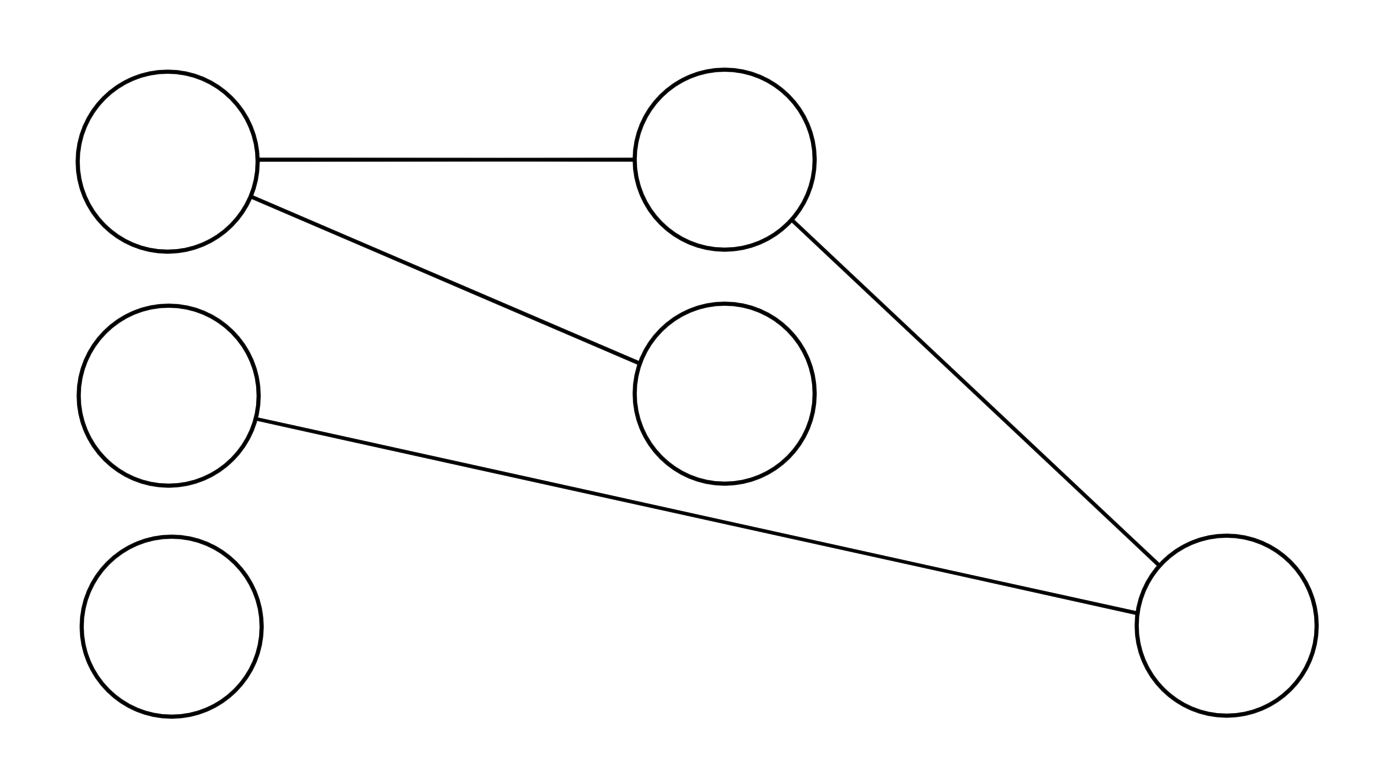
\includegraphics[width=0.5\textwidth]{figuras/ch_shift/shift-shift1.png}};
    \node at (1,3.6) {\large{$(1,2)$}};
    \node at (1,2.2) {\large{$(1,3)$}};
    \node at (1,0.8) {\large{$(1,4)$}};
    \node at (4.35,3.6) {\large{$(2,3)$}};
    \node at (4.35,2.2) {\large{$(2,4)$}};
    \node at (7.35,0.8) {\large{$(3,4)$}};
\end{tikzpicture}
\caption{O \textit{shift graph} $S_4$}
\label{fig:shiftgraph}
\end{figure}

\begin{definicao}
Um \textit{shift graph} de parâmetro $n$ e ordem $r$, denotado $S_n^r$, é um grafo cujos vértices são as $(r+1)$-uplas $(a_0, a_1, a_2, \cdots, a_r)$, onde $1 \leq a_0 < a_1 < \cdots < a_r \leq n$, e dois vértices $a = (a_0, \cdots, a_r)$ e $b = (b_0, \cdots, b_r)$ são adjacentes se $a\setminus a_0 = b\setminus b_r$ ou $a\setminus a_r = b\setminus b_0$, ou seja, se os $r$ primeiros elementos de um vértice coincidem com os $r$ últimos elementos do outro vértice.
\end{definicao}

\begin{figure}[H]
\centering
\begin{tikzpicture}
    \node[anchor=south west,inner sep=0] at (0,0) {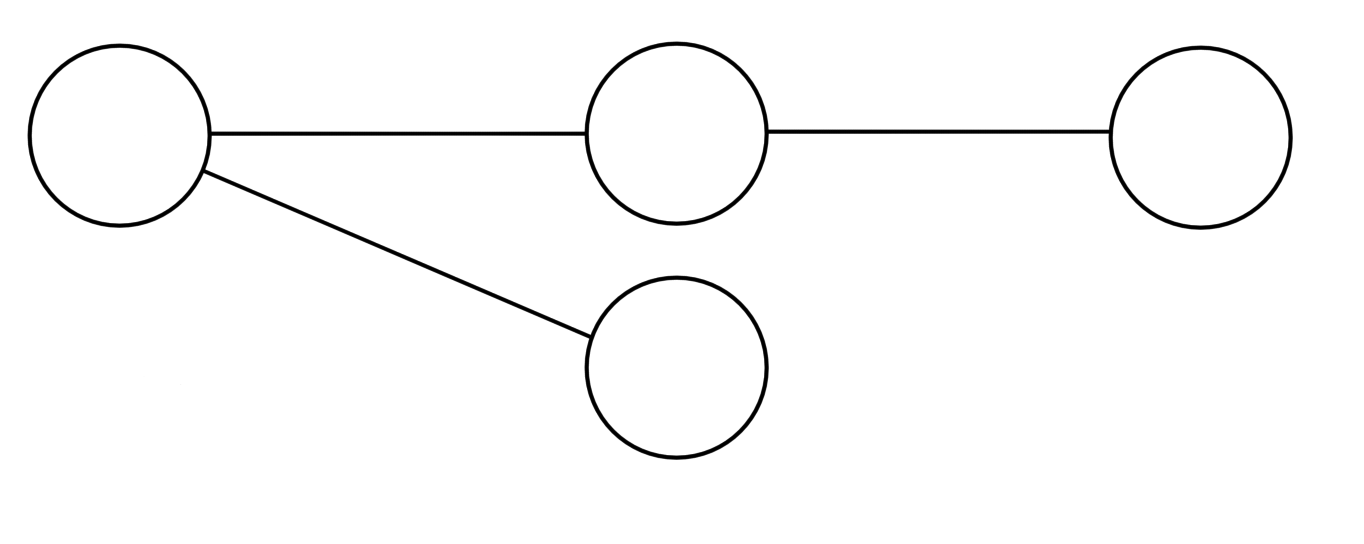
\includegraphics[width=0.6\textwidth]{figuras/ch_shift/shift-shiftorder2.png}};
    \node at (0.87,2.95) {$(1,2,3)$};
    \node at (4.9,2.95) {$(2,3,4)$};
    \node at (4.9,1.25) {$(2,3,5)$};
    \node at (8.7,2.95) {$(3,4,5)$};
\end{tikzpicture}
\caption{Alguns vértices de $S_5^{2}$}
\label{fig:shiftgraphorder2}
\end{figure}

\begin{definicao}
Dado um grafo $G$, o grafo linha de $G$, denotado por $L(G)$, é o grafo definido da seguinte forma
\[V(L(G)) = \{e : e \in E(G)\}\]
\[E(L(G)) = \{vw : v,w \in E(G) \text{ e } |v \cap w| = 1\},\]
ou seja, os vértices do grafo $L(G)$ são as arestas de $G$, e dois vértices de $L(G)$ são adjacentes se as arestas correspondentes em $G$ têm um vértice em comum.

Ademais, o digrafo linha $L(D)$ de um digrafo $D$ é definido da seguinte forma
\[V(L(D)) = \{a : a \in A(D)\}\]
\[A(L(D)) = \{vw : v,w \in A(D) \text{ e } vw \text{ é um caminho dirigido em D}\},\]
ou seja, os vértices de $L(D)$ são os arcos de $D$, e $vw$ é um arco em $L(D)$ se existe um vértice $x$ em $D$ tal que o arco $v$ entra em $x$, e o arco $w$ saia de $x$.
\end{definicao}

\begin{figure}[H]
\centering
\begin{tikzpicture}
    \node[anchor=south west,inner sep=0] at (0,0) {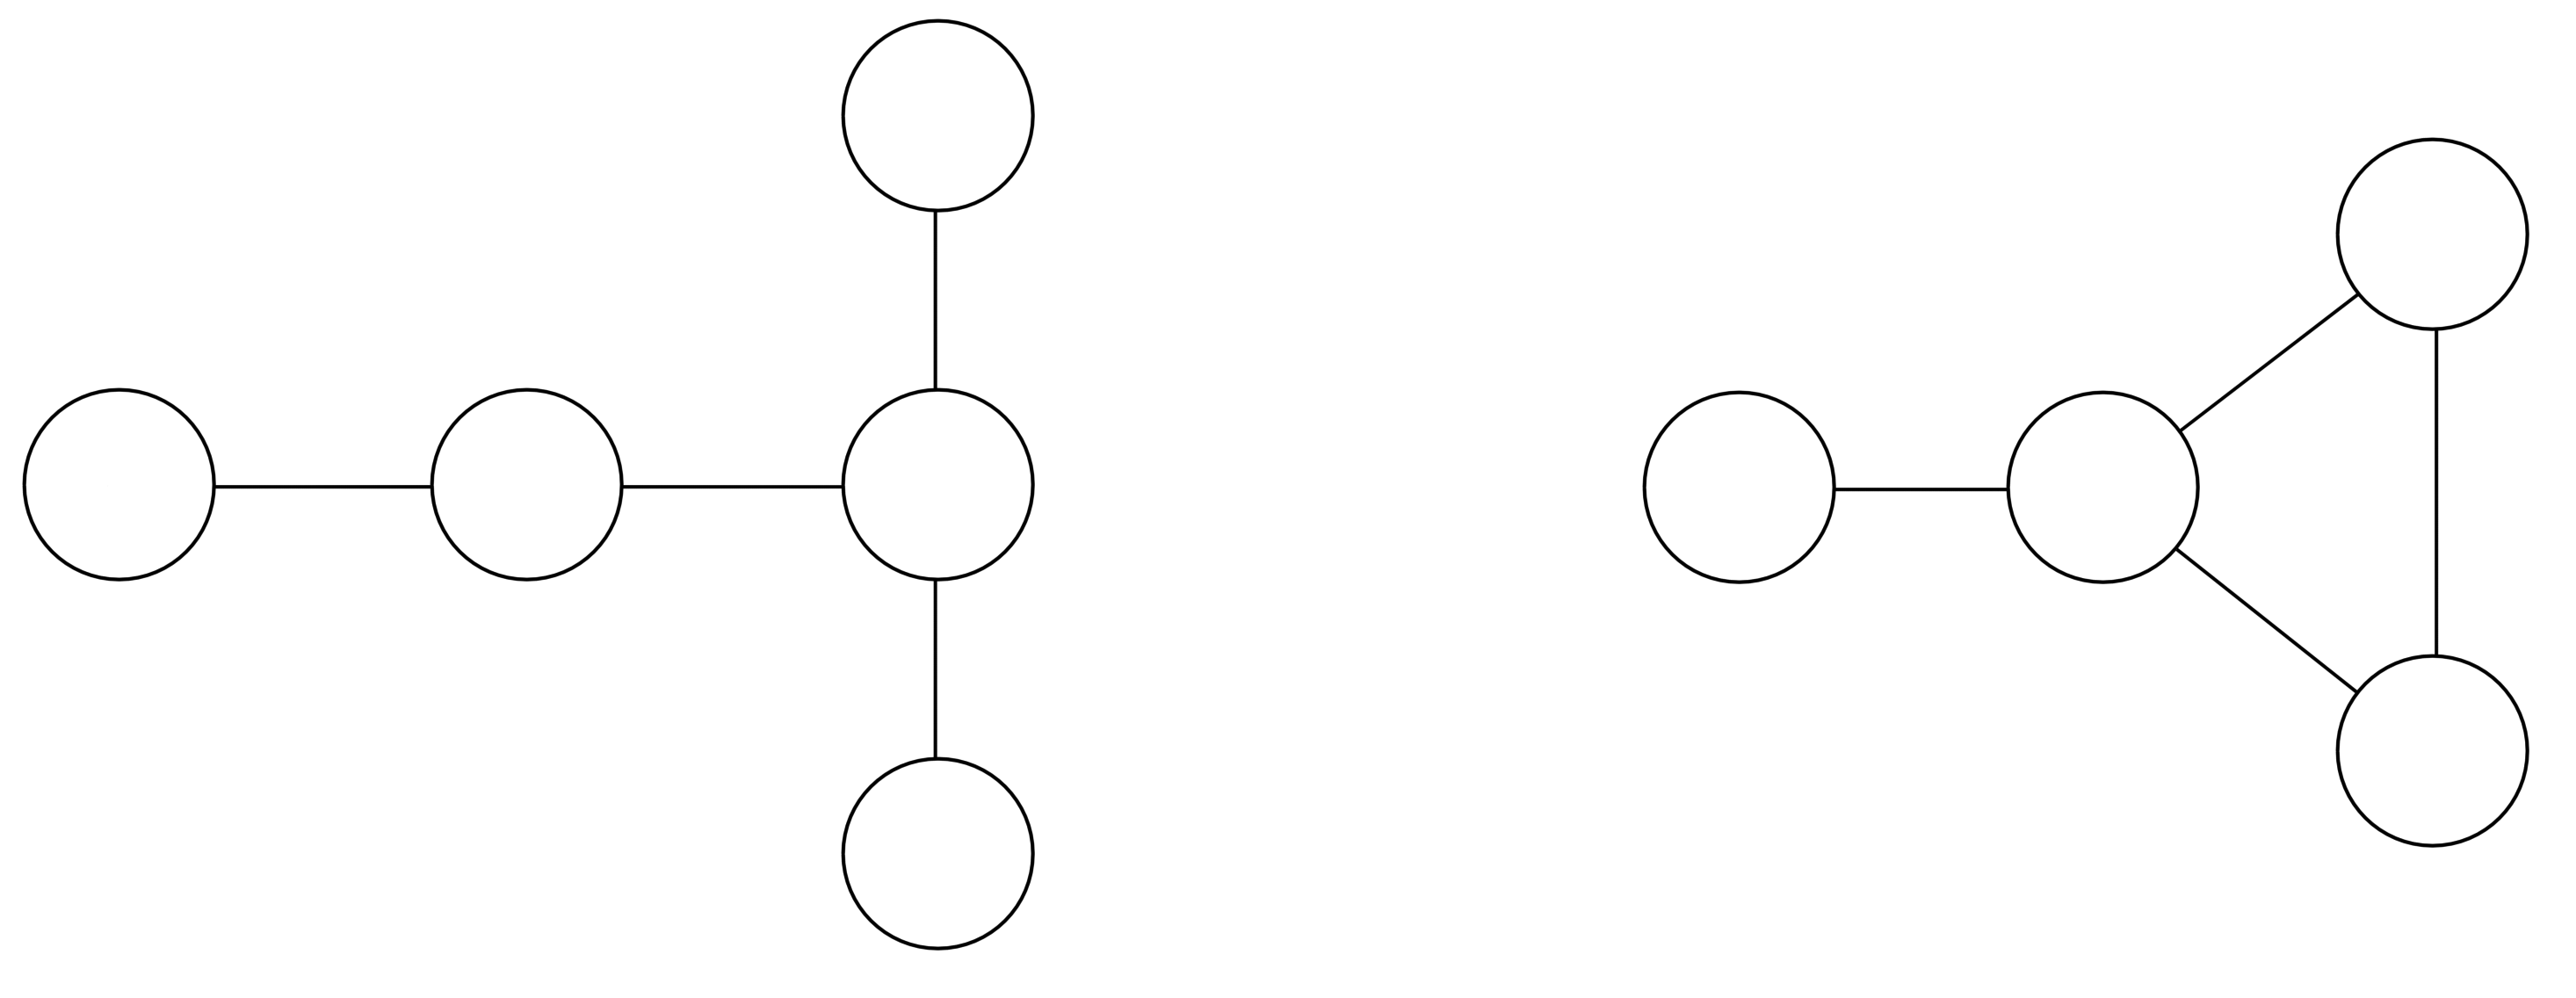
\includegraphics[width=0.85\textwidth]{figuras/ch_shift/shift-linegraph.png}};
    \node at (0.68,2.75) {\Large$v_1$};
    \node at (2.88,2.75) {\Large$v_2$};
    \node at (5.1,2.75) {\Large$v_3$};
    \node at (5.1,0.75) {\Large$v_4$};
    \node at (5.1,4.75) {\Large$v_5$};
    \node at (1.78,3.1) {\Large$e_1$};
    \node at (3.99,3.1) {\Large$e_2$};
    \node at (5.5,1.75) {\Large$e_3$};
    \node at (5.5,3.75) {\Large$e_4$};
    \node at (9.5,2.75) {\Large$e_1$};
    \node at (11.45,2.75) {\Large$e_2$};
    \node at (13.25,1.33) {\Large$e_3$};
    \node at (13.25,4.15) {\Large$e_4$};
\end{tikzpicture}
\caption{Um grafo $G$ (esquerda) e seu grafo linha $L(G)$ (direita).}
\label{fig:shiftlinegraph}
\end{figure}

\begin{figure}[H]
\centering
\begin{tikzpicture}
    \node[anchor=south west,inner sep=0] at (0.02,-0.07) {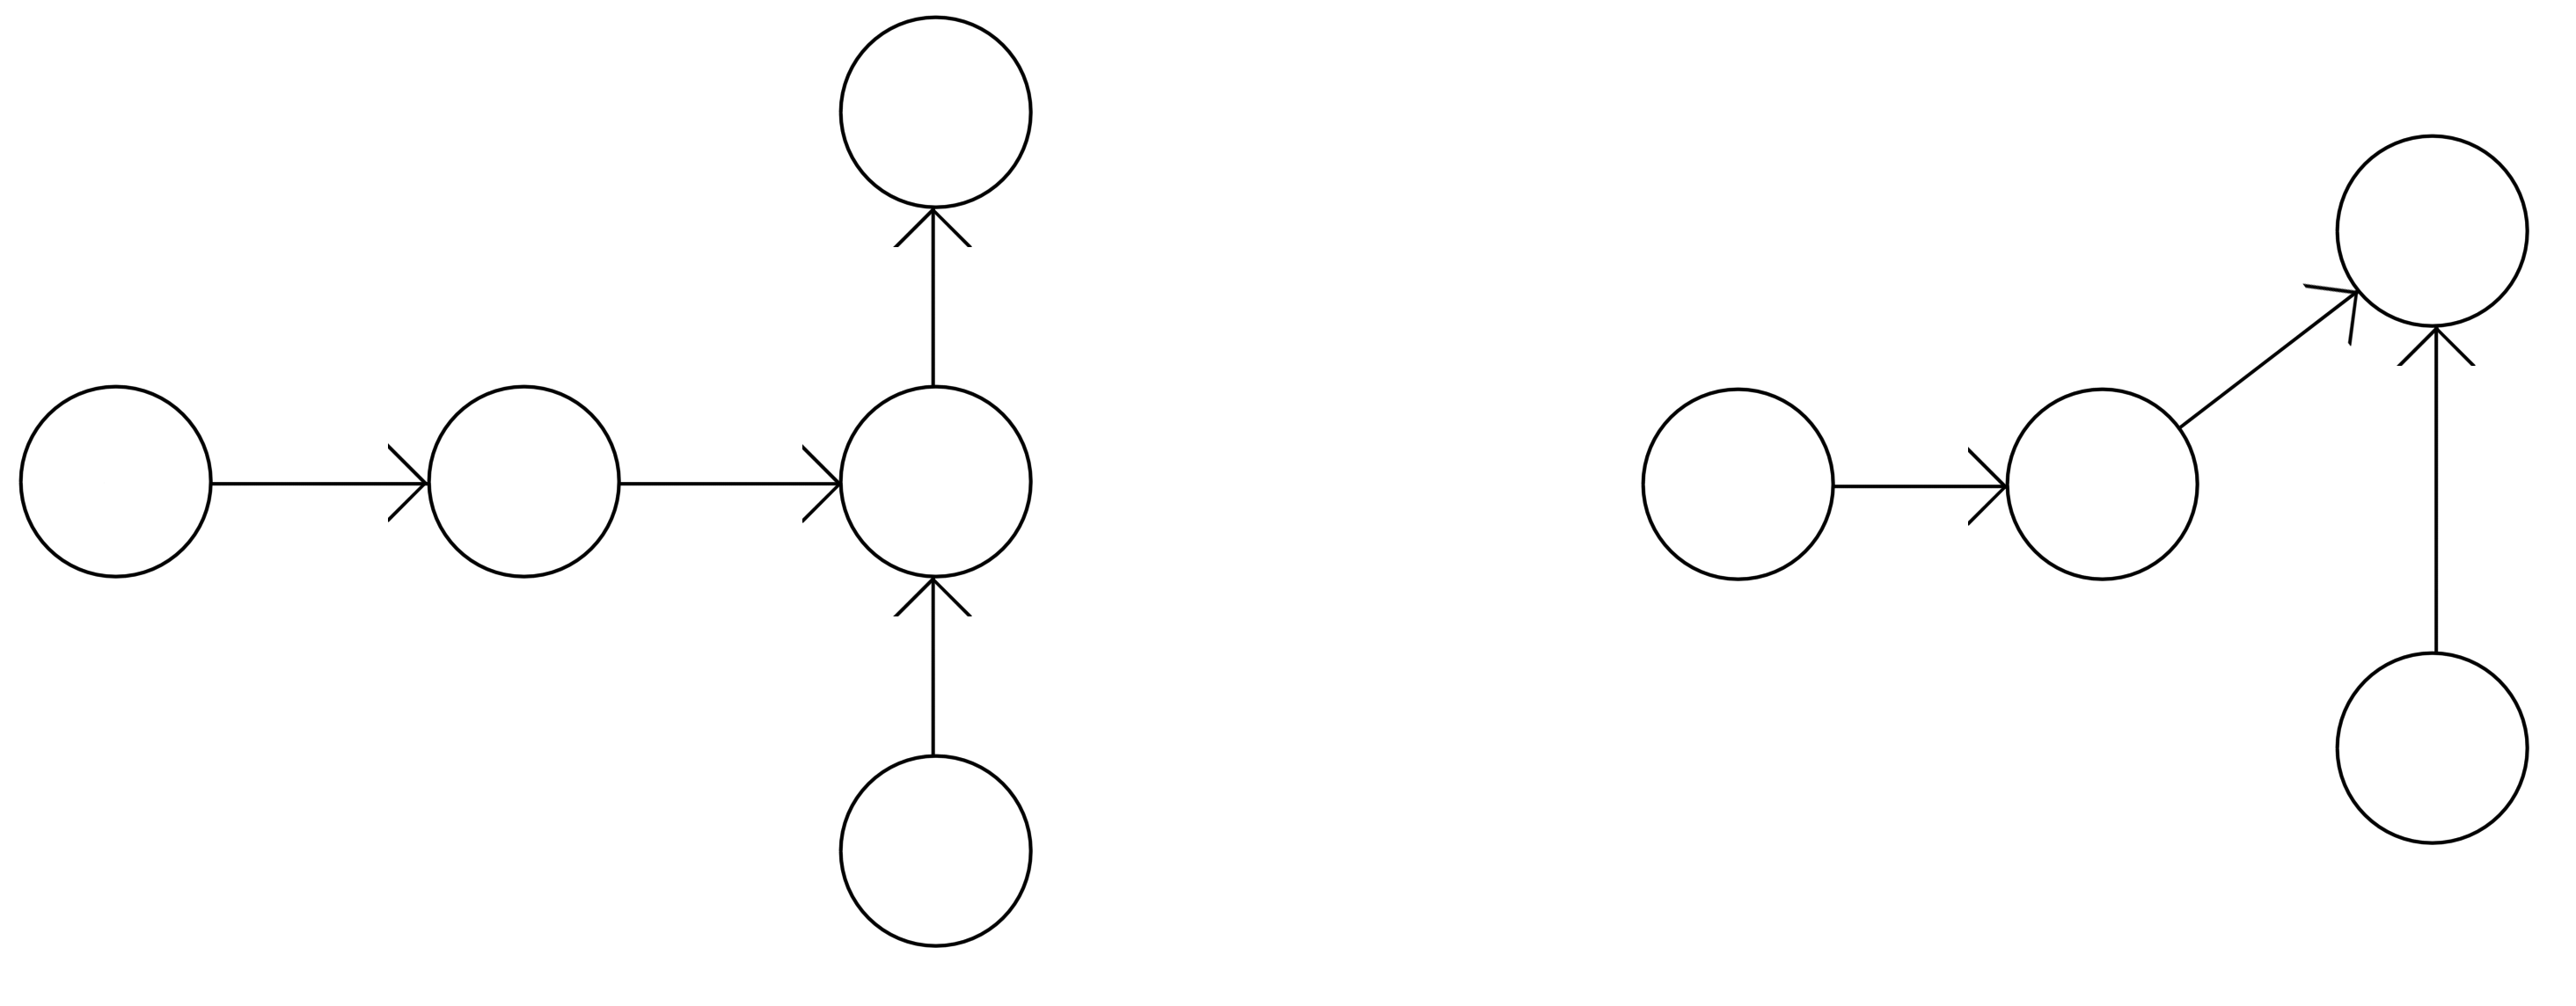
\includegraphics[width=0.85\textwidth]{figuras/ch_shift/shift-linedigraph.png}};
    \node at (0.68,2.75) {\Large$v_1$};
    \node at (2.88,2.75) {\Large$v_2$};
    \node at (5.1,2.75) {\Large$v_3$};
    \node at (5.1,0.75) {\Large$v_4$};
    \node at (5.1,4.75) {\Large$v_5$};
    \node at (1.78,3.1) {\Large$a_1$};
    \node at (3.99,3.1) {\Large$a_2$};
    \node at (5.5,1.75) {\Large$a_3$};
    \node at (5.5,3.75) {\Large$a_4$};
    \node at (9.5,2.75) {\Large$a_1$};
    \node at (11.45,2.75) {\Large$a_2$};
    \node at (13.25,1.33) {\Large$a_3$};
    \node at (13.25,4.15) {\Large$a_4$};
\end{tikzpicture}
\caption{Um digrafo $D$ (esquerda) e seu digrafo linha $L(D)$ (direita).}
\label{fig:shiftlinedigraph}
\end{figure}

Seja $L^1(G) := L(G)$, e para $r>1$ seja $L^r(G) := L(L^{r-1}(G))$. Denotamos $S_n^0 := K_n$ e $L^0(G) := G$. 

\begin{teorema}\label{shiftteo}
A família dos \textit{shift graphs} de ordem $r$ respeita a conjectura de Erd\H{o}s e Hajnal. \cite{gabor2018cepa}
\end{teorema}

\section{Número Cromático}

\begin{afirmacao}\label{shiftchraff1}
O número cromático do \textit{shift graph} $S_n$ é $\ceil{\log_2(n)}$.
\end{afirmacao}

\begin{proof}(Afirmação \ref{shiftchraff1})
Seja $D$ uma orientação transitiva de $K_n$. Temos que $S_n$ é uma simetrização de $L(D)$. Para mostrar que $\chi(S_n) \geq \ceil{\log_2(n)}$, suponha que $S_n$ pode ser colorido com $\ceil{\log_2(n)} - 1$ cores e tome uma $(\ceil{\log_2(n)} -1)$-coloração de $S_n$. Tal coloração dos vértices de $S_n$ corresponde a uma $(\ceil{\log_2(n)}-1)$-coloração dos arcos de $D$. Para cada vértice de $D$ atribua um vetor binário tal que cada entrada corresponda a uma das $\ceil{\log_2(n)}-1$ cores dos arcos, e cada entrada tem valor $1$ se algum arco da cor correspondente chega no vértice, e $0$ caso contrário. 

Temos que tal coloração é própria, pois caso exista um arco $vw$ monocromático em $D$, temos que existe um arco que chega em $v$ com a mesma cor do arco entre $v$ e $w$, o que não é possível, pois tal configuração é um arco monocromático em $L(D)$. 

E temos que tal coloração usa $2^{(\ceil{\log_2(n)}-1)} < n$ cores, contradição, pois $D$ é um digrafo completo, e logo precisa de $n$ cores.
\end{proof}

O número cromático de $S_n$ é $\ceil{\log_2(n)}$. De forma geral, o número cromático de $S_n^r$ é $(1+o(1))\log_2 \log_2 \cdots \log_2 (n)$, onde o logaritmo é tomado $r$ vezes \cite{erdos1968chromatic}.

%%%%%%%%%%%%%%%%%%%%%%%%%%%%%%%%%%%%%%%%%%%%%%%%%%%%%%%%%%%%%%%%%%%%%%%%%%%%%
% ^ Escrever onde quer chegar com isso
%%%%

\section{Esboço da prova}

Seja $D$ uma orientação transitiva de $K_n$. Mostraremos que $L^r(D)$ é isomorfo a um direcionamento de $S_n^r$. Aplicando o Lema Local de Lovász, encontraremos em $S_n^r$ um subgrafo $H$ tal que $H$ tem cintura grande e contém pelo menos uma aresta de cada $K_{d,d}$ de $S_n^r$.

Queremos então mostrar que o número cromático de $H$ não é limitado por uma constante, ou seja, $\chi(H) \rightarrow \infty$ conforme $n \rightarrow \infty$.

Provaremos que se temos uma $t$-coloração de $S_n^r$ sem $K_{d,d}$ monocromático, existe uma $2^t$-coloração de $S_n^{r-1}$ sem $K_{td,td}$ monocromático. E logo, existe uma $t'$-coloração de $S_n^i$ sem $K_{d',d'}$ monocromático para cada $i\in [0,r]$, para algum par de inteiros $t'$ e $d'$.

Uma coloração própria de $H$ é uma coloração de $S_n^r$ sem $K_{d,d}$ monocromático. Então suponha que o número cromático de $H$ é limitado por uma constante, existem constantes $t'$ e $d'$ tais que $S_n^i$ pode ser $t'$-colorido sem $K_{d',d'}$ monocromático, em particular, existe tal coloração para $S_n^0 = D$. Contradição, pois note que um conjunto de $2d'$ vértices coloridos com uma mesma cor é um $K_{d',d'}$ monocromático em $D$, e com apenas $t' < \infty$ cores, alguma cor ocorre pelo menos $2d'$ vezes em $D$ conforme $n\rightarrow\infty$. Logo o número cromático de $H$ não é limitado por uma contante.

\section{Prova do Teorema}

\begin{afirmacao}\label{shiftafirm1}
Seja $D$ uma orientação transitiva de $K_n$. Então $S_n^r$ é uma simetrização de $L^r(D)$.
\end{afirmacao}

\begin{proof}(Afirmação \ref{shiftafirm1})
Seja $V(D) = \{1,2,\cdots, n\}$, onde para cada $i < j$, existe um arco de $i$ para $j$. Mostraremos que a simetrização de $L(D)$ é isomorfa a $S_n^1$.

Denotemos por $(i,j)$ os arcos de $D$, onde $i < j$. Logo os vértices de $L(D)$ são os pares $(i,j)$ com $i < j$. E para cada $1 \leq i < j < k \leq n$, existe em $D$ um arco de $i$ para $j$ e um arco de $j$ para $k$. Logo em $L(D)$ existe um arco de $(i,j)$ para $(j,k)$. Temos então que

\[V(L(D)) = \{(i,j) : 1\leq i < j \leq n\},\]
\[A(L(D)) = \{(i,j)(j,k) : 1\leq i <j<k\leq n\}.\]

E temos que $S_n^1$ tem como conjunto de vértices os pares $(i,j)$ com $1\leq i<j\leq n$. E dois vértices $(a,b)$ e $(c,d)$ são adjacentes se $a = d$ ou $b = c$. Logo temos que

\[V(S_n^1) = \{(i,j) : 1\leq i<j\leq n\},\]
\[E(S_n^1) = \{(i,j)(j,k) : 1\leq i<j<k\leq n\}.\]

Temos portanto que $L(D)$ e $S_n^1$ são ``quase isomorfos'', exceto pelo fato de que $L(D)$ é direcionado, portanto $S_n^1$ é uma simetrização de $L(D)$.

%Denotemos por $(i,j)$ os arcos de $D$, onde $i < j$. Então os vértices de $L(D)$ são os pares $(i,j), i<j$. E os vértices de $S_n^1$ são os pares $(i,j), 1\leq i < j \leq n$. Claramente existe uma bijeção entre os vértices de $L(D)$ e os vértices de $S_n^1$.

%Para cada $1\leq i < j < k \leq n$, existe em $D$ um arco de $i$ para $j$ e um arco de $j$ para $k$, logo em $L(D)$ existe um arco de $(i,j)$ para $(j,k)$. E em $S_n^1$, para cada $1\leq i < j < k \leq n$ existe uma aresta entre $(i,j)$ e $(j,k)$. Claramente existe uma bijeção entre os arcos de $L(D)$ e as arestas de $S_n^1$. Temos portanto que $L(D)$ e $S_n^1$ são ``quase isomorfos'', exceto pelo fato de que $L(D)$ é direcionado, portanto $S_n^1$ é uma simetrização de $L(D)$.

De forma semelhante, mostraremos que $S_n^r$ é uma simetrização de $L^r(D)$ para $r>1$.

Temos que $L^r(D) = L(L^{r-1}(D))$, e como $L^{r-1}(D)$ é um direcionamento de $S_n^{r-1}$, sabemos que os vértices de $L^{r-1}(D)$ são as $r$-uplas $(v_0,\cdots,v_{r-1})$, onde $1\leq v_0 < \cdots < v_{r-1} \leq n$, e temos que para cada escolha de $1\leq v_0 < \cdots < v_{r} \leq n$, existe um arco de $(v_0,\cdots,v_{r-1})$ para $(v_1,\cdots,v_r)$.

Para cada $1\leq v_0 < \cdots < v_{r} \leq n$, denote por $(v_0,\cdots,v_{r})$ o arco de $(v_0,\cdots,v_{r-1})$ para $(v_1,\cdots,v_r)$ em $L^{r-1}(D)$. Portanto $L(L^{r-1}(D))$ tem como vértices as $(r+1)$-uplas $(v_0,\cdots,v_{r})$, onde $1\leq v_0 < \cdots < v_r \leq n$.

Temos que para cada $1\leq v_0 < \cdots < v_{r+1} \leq n$, existe em $L^{r-1}(D)$ um arco de $(v_0,\cdots,v_{r-1})$ para $(v_1,\cdots,v_r)$ e um arco de $(v_1,\cdots,v_{r})$ para $(v_2,\cdots,v_{r+1})$. Logo em $L(L^{r-1}(D))$, para cada $1\leq v_0 < \cdots < v_{r+1} \leq n$ existe um arco de $(v_0,\cdots,v_{r})$ para $(v_1,\cdots,v_{r+1})$. Logo

\[V(L^r(D)) = \{(v_0,\cdots,v_{r}) : 1\leq v_0 < \cdots < v_r \leq n\},\]
\[A(L^r(D)) = \{(v_0,\cdots,v_{r})(v_1,\cdots,v_{r+1}) : 1\leq v_0 < \cdots < v_{r+1} \leq n\}.\]

E os vértices de $S_n^r$ são as $(r+1)$-uplas $(v_0, v_1, \cdots, v_r)$, onde $1\leq v_0 < v_1 < \cdots < v_r \leq n$. E para cada $1 \leq v_0 < v_1 <\cdots < v_r < v_{r+1} \leq n$, os vértices $(v_0, \cdots, v_r)$ e $(v_1, \cdots, v_{r+1})$ são adjacentes. Então 

\[V(S_n^r) = \{(v_0, v_1, \cdots, v_r) : 1 \leq v_0 < \cdots < v_r \leq n\},\]
\[E(S_n^r) = \{(v_0, v_1, \cdots, v_r)(v_1, v_2, \cdots, v_{r+1}) : 1 \leq v_0 < \cdots < v_{r+1} \leq n\}.\]

%Temos que $L^r(D) = L(L^{r-1}(D))$, e como $L^{r-1}(D)$ é um direcionamento de $S_n^{r-1}$, sabemos que os vértices de $L^{r-1}(D)$ são as $r$-uplas $(v_0,\cdots,v_{r-1})$, onde $1\leq v_0 < \cdots < v_{r-1} \leq n$, e temos que para cada escolha de $1\leq v_0 < \cdots < v_{r} \leq n$, existe um arco de $(v_0,\cdots,v_{r-1})$ para $(v_1,\cdots,v_r)$.

%Então para cada $1\leq v_0 < \cdots < v_{r} \leq n$, denote por $(v_0,\cdots,v_{r})$ o arco de $(v_0,\cdots,v_{r-1})$ para $(v_1,\cdots,v_r)$ em $L^{r-1}(D)$. Portanto temos uma bijeção entre os vértices de $L(L^{r-1}(D))$ e os vértices de $S_n^r$.

%E para cada $1\leq v_0 < \cdots < v_{r+1} \leq n$, existe em $L^{r-1}(D)$ um arco de $(v_0,\cdots,v_{r-1})$ para $(v_1,\cdots,v_r)$ e um arco de $(v_1,\cdots,v_{r})$ para $(v_2,\cdots,v_{r+1})$. Logo em $L(L^{r-1}(D))$, para cada $1\leq v_0 < \cdots < v_{r+1} \leq n$ existe um arco de $(v_0,\cdots,v_{r})$ para $(v_1,\cdots,v_{r+1})$.

Temos portanto que $S_n^r$ é uma simetrização de $L^r(D)$.
\end{proof}

\begin{lema}\label{shiftlema1}
Seja $D$ um grafo dirigido. Se $L(D)$ pode ser colorido com $t$ cores sem $K_{d,d}$ monocromático, então $D$ pode ser colorido com $2^t$ cores sem $K_{td,td}$ monocromático.
\end{lema}

\begin{proof}{(Lema \ref{shiftlema1})}
Considere uma $t$-coloração de $L(D)$ sem $K_{d,d}$ monocromático. Tal coloração corresponde a uma coloração dos arcos de $D$ com $t$ cores.

Considere a seguinte coloração dos vértices de $D$. Cada vértice é colorido com um vetor binário de $t$ entradas, correspondentes às $t$ cores dos arcos, onde cada entrada é $1$ caso entrem pelo menos $d$ arcos da cor correspondente, e $0$ caso contrário.

\begin{figure}[H]
\centering
\begin{tikzpicture}
    \node[anchor=south west,inner sep=0] at (0.02,-0.07) {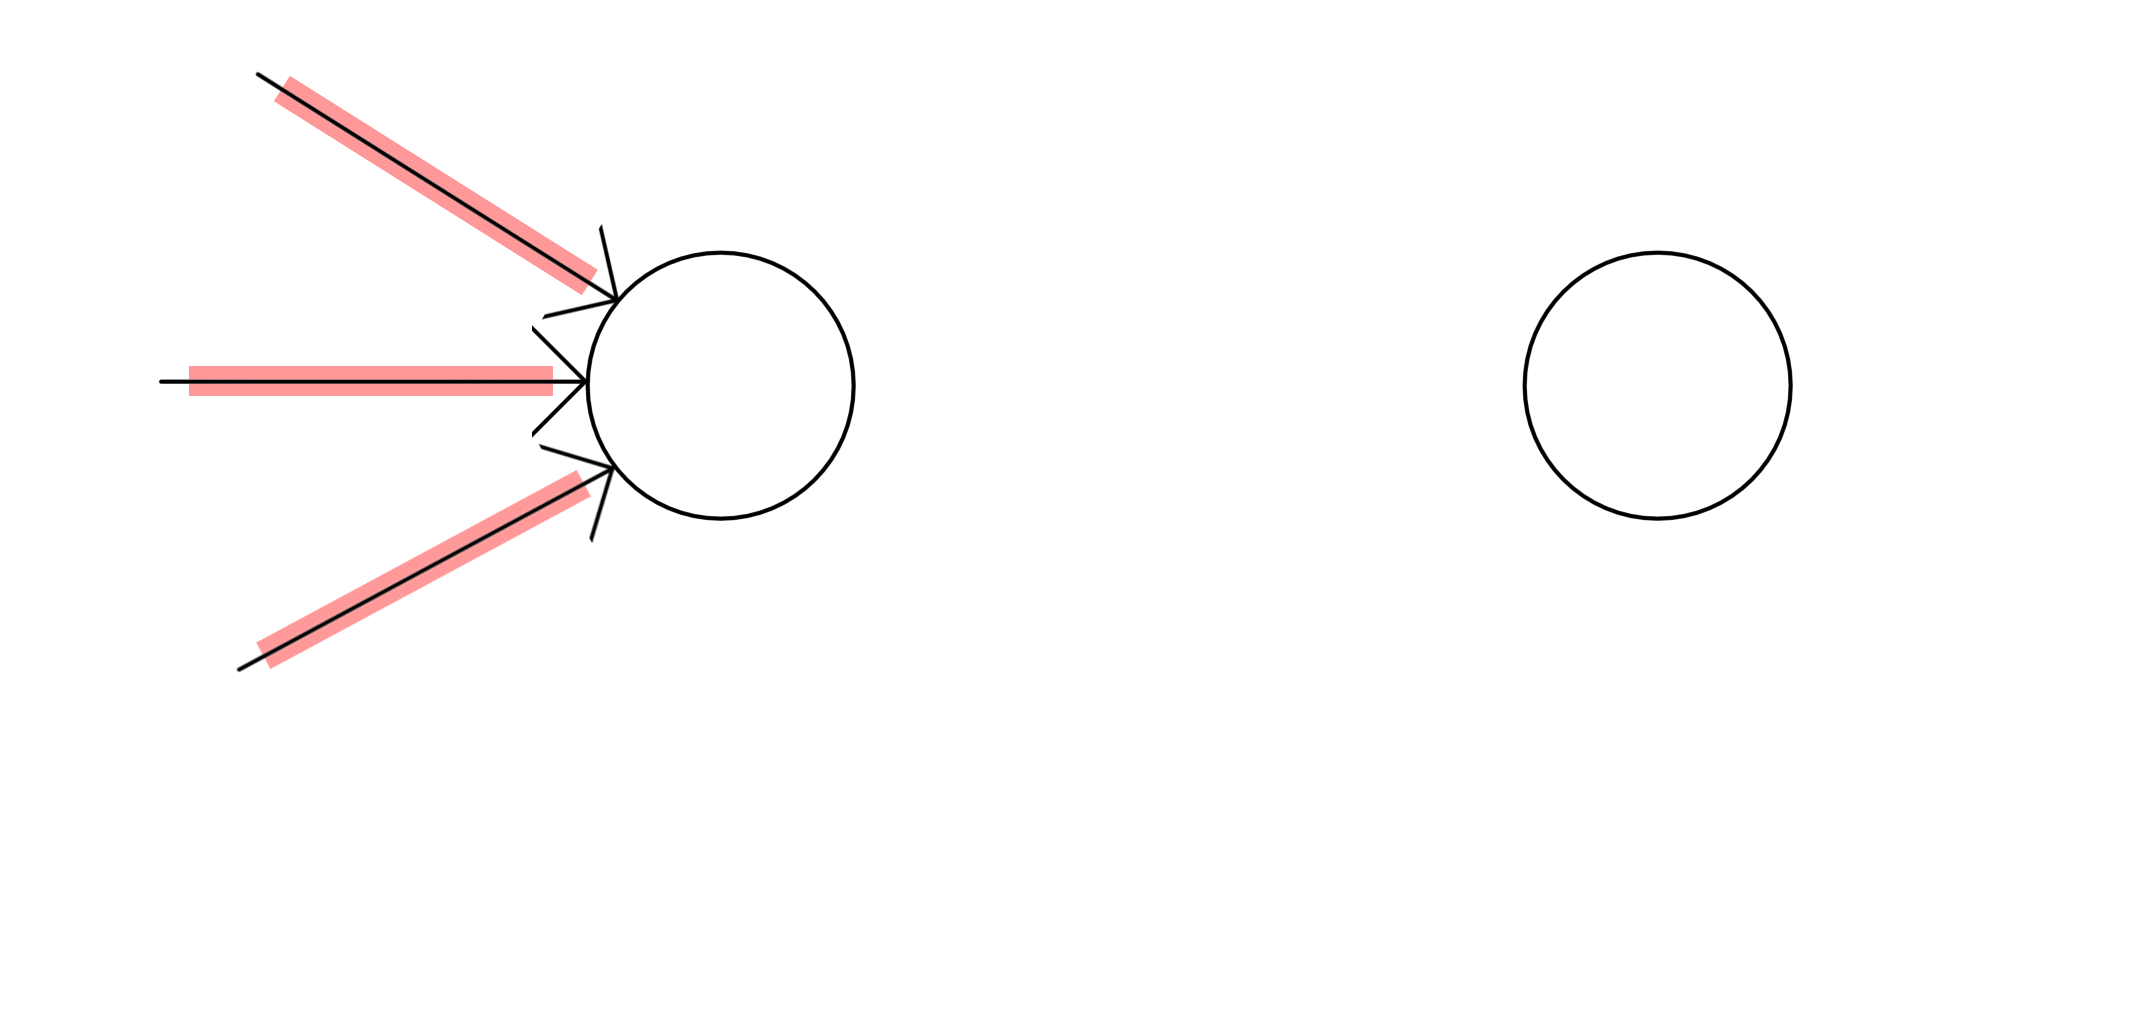
\includegraphics[width=0.85\textwidth]{figuras/ch_shift/shift-arccoloringtovertex.png}};
    \node at (10.85,1.6) {\large$(\cdots, 1, \cdots)$};
    \node at (10.85,1.0) {\large$i$};
    \draw [decorate,decoration={brace,amplitude=10pt},xshift=0pt,yshift=0pt](4.0,1.6) -- (0.8,1.6) node [black,midway,yshift=-0.6cm] {$\geq d$ arcos de cor $i$.};
\end{tikzpicture}
\caption{A $i$-ésima entrada da cor de um vértice é $1$ se nele entram pelo menos $d$ arcos de cor $i$.}
\label{fig:shiftarccoloringtovertex}
\end{figure}

Mostraremos que esta coloração é tal como descrita pelo lema. 

Claramente, temos no máximo $2^t$ cores. Então basta mostrar que tal coloração não contém $K_{td,td}$ monocromático.

Suponha por contradição que existe $K_{td,td}$ monocromático de cor $v$, e digamos que os arcos vão do conjunto de vértices $A$ para o conjunto de vértices $B$. Seja $k$ o número de entradas $0$ em $v$. Para cada vértice de $B$, sabemos que chegam no máximo $d-1$ arcos com cada uma das $k$ cores de entrada $0$ em $v$, pois caso contrário tal cor não teria entrada $0$ em $v$. Logo, no máximo $ktd(d-1)$ arcos do $K_{td,td}$ tem uma das $k$ cores de entrada $0$. Portanto, temos pelo menos $t^2d^2 - ktd(d-1) = td(td - k(d-1))$ arcos com uma das $t-k$ cores de entrada $1$ em $v$.

Como temos $|A| = td$ e $td(td - k(d-1))$ arcos com uma das cores de entrada $1$, pelo principio da casa dos pombos, de algum vértice de $A$ saem pelo menos $td - k(d-1) = d(t-k) + k$ arcos com uma das cores de entrada $1$. E como temos $t-k$ cores com entrada $1$, alguma delas ocorre pelo menos $d + k/(t-k)$ vezes. 

Temos portanto que de algum vértice de $A$ saem pelo menos $d$ arcos com uma cor de entrada $1$, e entram pelo menos $d$ arcos da mesma cor (pois tal cor tem entrada $1$ em $v$). Tal configuração corresponde a um $K_{d,d}$ monocromático em $L(D)$, contradição.

\begin{figure}[H]
\centering
\begin{tikzpicture}
    \node[anchor=south west,inner sep=0] at (0,0) {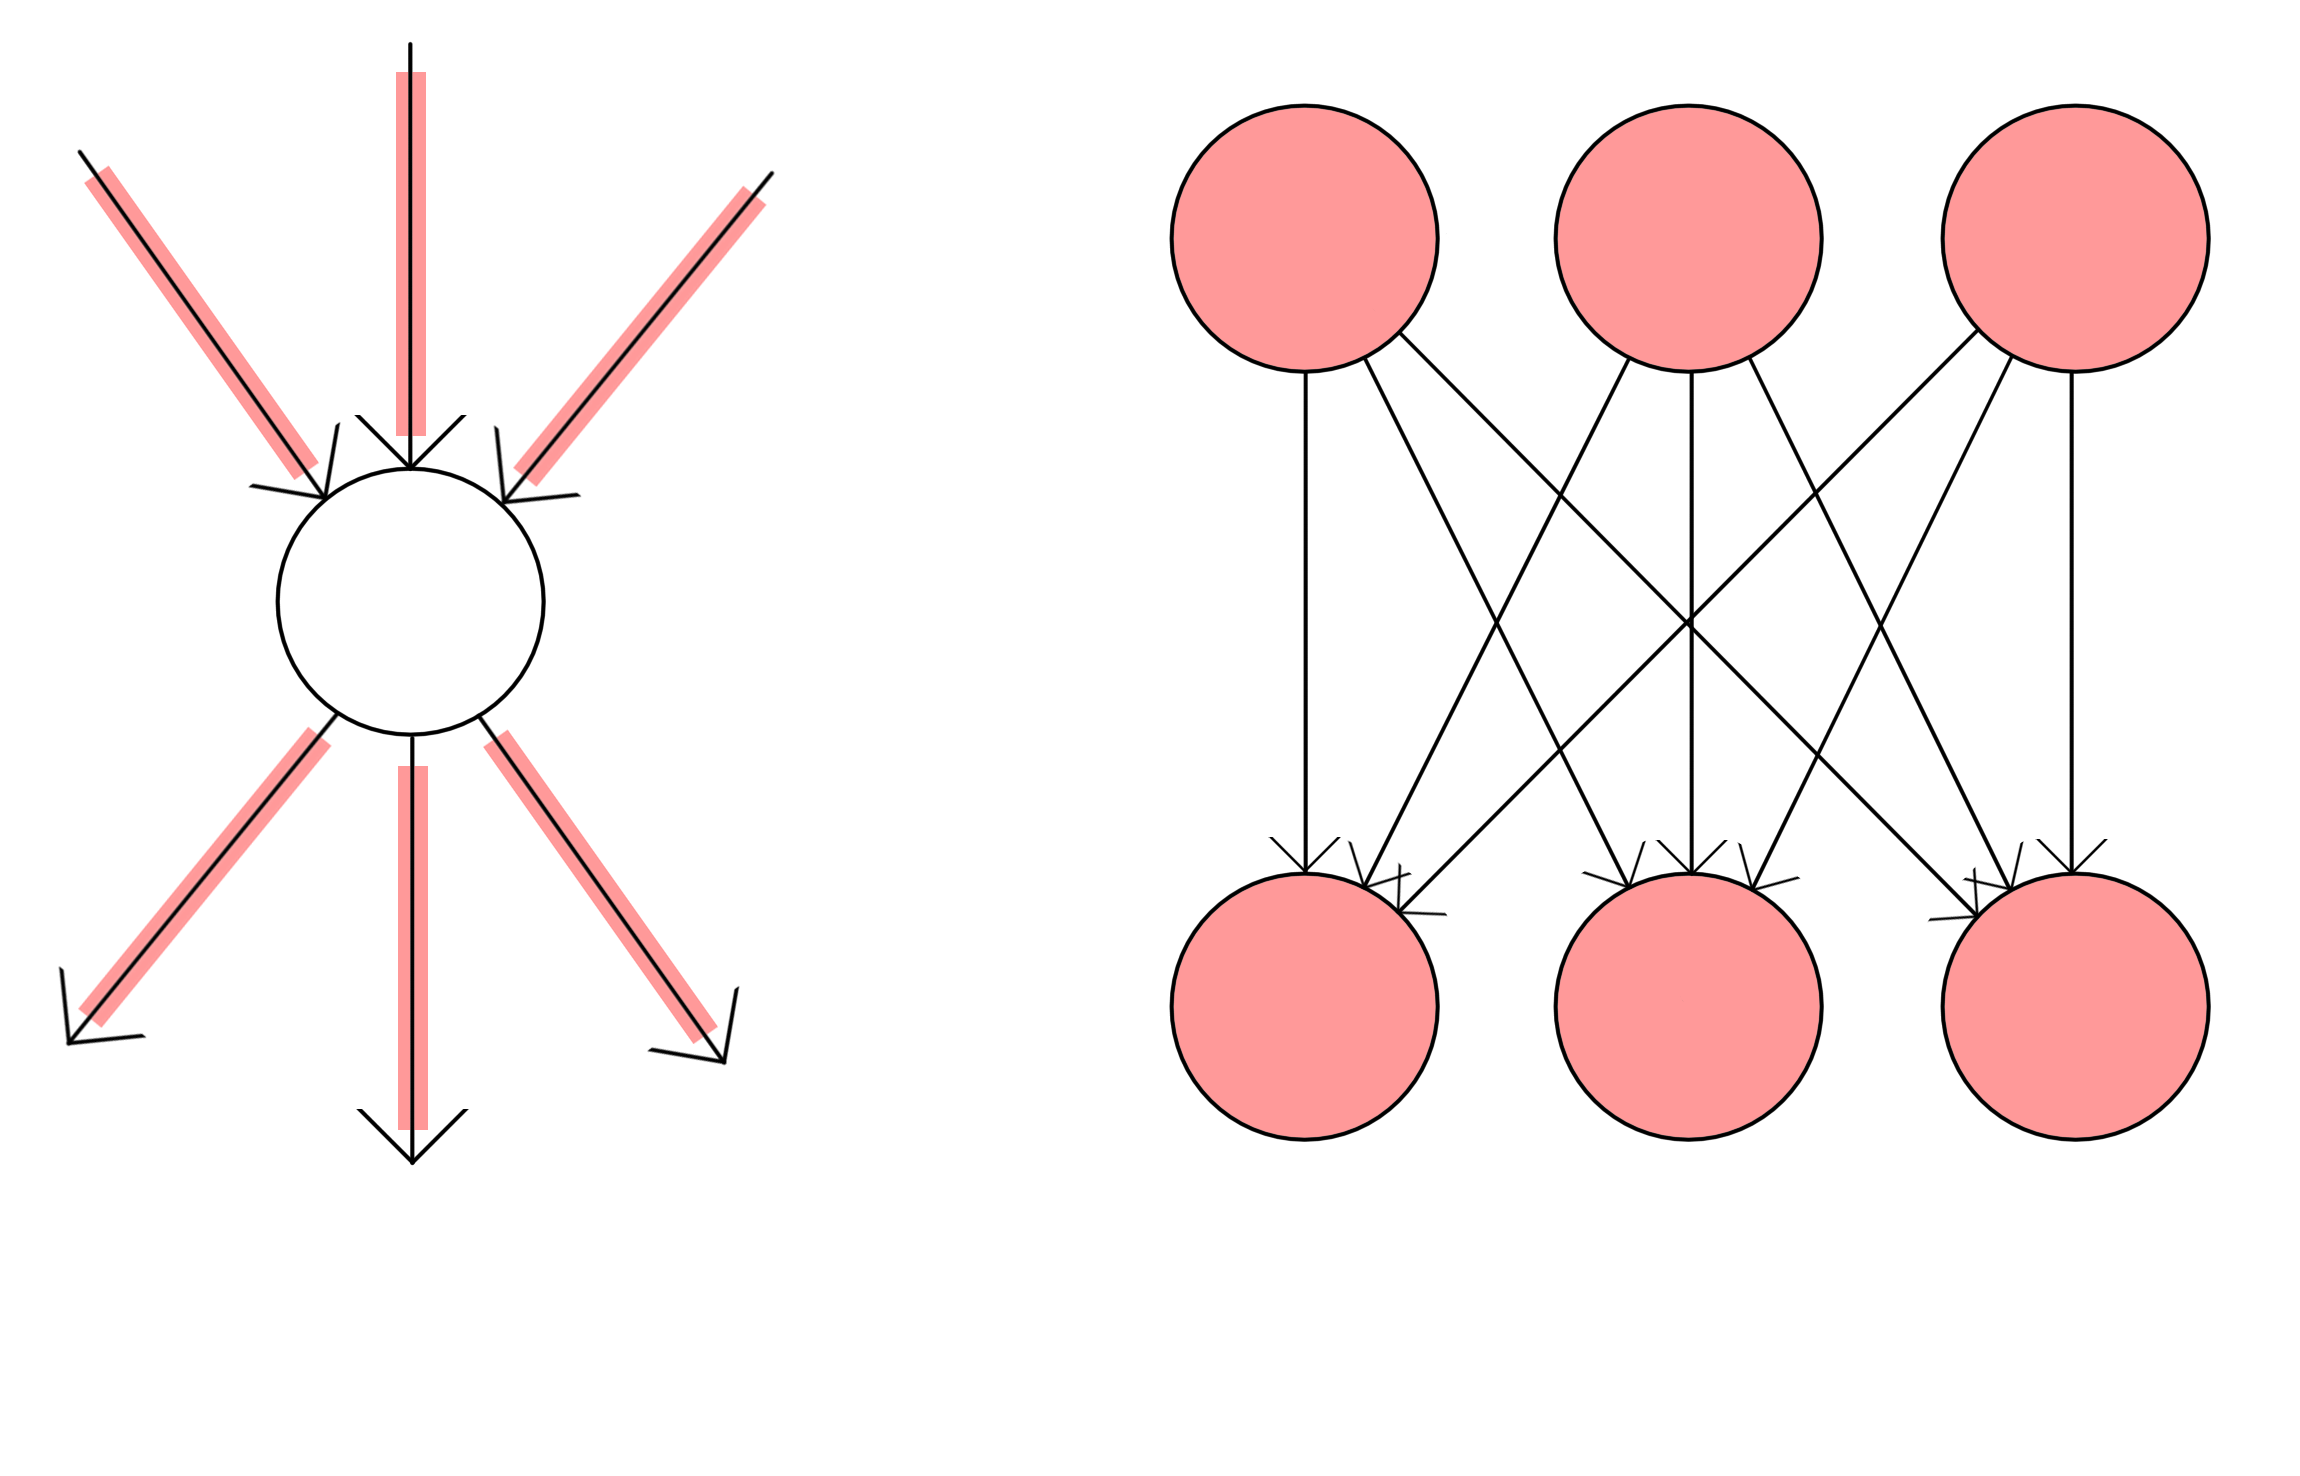
\includegraphics[width=0.75\textwidth]{figuras/ch_shift/shift-kdd.png}};
    \node at (2.2,1) {\large$D$};
    \node at (9.2,1) {\large$L(D)$};
\end{tikzpicture}
\caption{Um vértice de $D$ com $d$ arcos de mesma cor entrando e saindo corresponde a um $K_{d,d}$ monocromático em $L(D)$.}
\label{fig:shiftkdd}
\end{figure}

Note que $t=k$ (ou seja, $v$ é composto apenas de zeros) não ocorre, pois em cada vértice de $B$ entram $td$ arcos de $t$ possíveis cores, logo alguma cor ocorre pelo menos $d$ vezes, contradizendo o fato de que $v$ é composto apenas de zeros.
\end{proof}

\begin{lema}\label{shiftlema2}
Existe um subgrafo $H$ de $S_n^r$ com cintura pelo menos $g$ e contendo pelo menos uma aresta de cada $K_{d,d}$ de $S_n^r$.
\end{lema}

\begin{proof}(Lema \ref{shiftlema2})
Seja $\lambda = 1/4g$, $\theta = (g-2)/(g-1.75)$, $d = n^\theta$ e $p = d^{\lambda-1}$. Seja $H$ um subgrafo aleatório de $S_n^r$ em que cada aresta é escolhida com probabilidade $p$, e seja $\Delta = \Delta(S_n^r) = n-r-1$.
Demonstraremos usando o Lema Local de Lovász que com probabilidade positiva $H$ tem cintura pelo menos $g$ e contém uma aresta de cada $K_{d,d}$.

Para cada circuito $C$ de $S_n^r$ com $|C| \leq g$, seja $A_C$ o evento de todas as arestas de $C$ estarem em $H$. Então temos que \[\bbp(A_C) = p^{|C|}.\]

Para cada subgrafo $B$ isomorfo a $K_{d,d}$ de $S_n^r$, seja $A_B$ o evento de nenhuma aresta de $B$ estar em $H$. Então \[\bbp(A_B) = (1-p)^{d^2} \leq e^{pd^2} = e^{-d^{1+\lambda}}.\]

Cada circuito $C$ compartilha aresta com no máximo $|C|\Delta^{j-2}$ circuitos de comprimento $j$, e compartilha aresta com no máximo $|C|\binom{\Delta}{d}^2$ subgrafos $B$ isomorfos a $K_{d,d}$.

Cada subgrafo $B$ compartilha aresta com no máximo $d^2\Delta^{j-2}$ circuitos de comprimento $j$, e compartilha aresta com no máximo $\binom{\Delta}{d}^2$ subgrafos isomorfos a $K_{d,d}$.

Sejam $y_{|C|} = \bbp(A_C)^{1-\lambda}$ e $y_0 = y(B) = e^{-0.5d^{1+\lambda}}$. Queremos mostrar que

\begin{equation*}
\bbp(A_C) \leq y_{|C|}\left(\prod_{3\leq j\leq g}(1-y_j)^{|C|\Delta^{j-2}}\right)(1-y_0)^{|C|\binom{\Delta}{d}^2},
\end{equation*}
\begin{equation*}
\bbp(A_B)\leq y_0 \left(\prod_{3\leq j\leq g}(1-y_j)^{d^2\Delta^{j-2}}\right)(1-y_0)^{\binom{\Delta}{d}^2}.
\end{equation*}

%%%%%%%%%%%%%%%%%%%%%%%%%%%%%%%%%%%%%%%%%%%%%%%%%%%%%%%%%%%%%%%%%%%
Temos que $\Delta < n$, portanto basta mostrar que

\begin{equation}\label{shiftllleq1}
\bbp(A_C) \leq y_{|C|}\left(\prod_{3\leq j\leq g}(1-y_j)^{|C|n^{j-2}}\right)(1-y_0)^{|C|\binom{n}{d}^2},
\end{equation}
\begin{equation}\label{shiftllleq2}
\bbp(A_B)\leq y_0 \left(\prod_{3\leq j\leq g}(1-y_j)^{d^2n^{j-2}}\right)(1-y_0)^{\binom{n}{d}^2}.
\end{equation}

Para mostrar a inequação (\ref{shiftllleq1}), tomamos seu logaritmo

\[\log(\bbp(A_C)) \leq \log(\bbp(A_C)^{1-\lambda}) + \sum\limits_{3\leq j\leq g}|C|n^{j-2}\log(1-y_j)+|C|\binom{n}{d}^2\log(1-y_0).\]

Então basta mostrar que

\[|C|(\lambda-1)\log(d) \leq -(1-\lambda)^2|C|\log(d) + \sum\limits_{3\leq j\leq g}|C|n^{j-2}\log(1-y_j)+|C|\binom{n}{d}^2\log(1-y_0).\]

Podemos dividir todos os termos por $|C|$ para obter

\[(\lambda-1)\log(d) \leq -(1-\lambda)^2\log(d) + \sum\limits_{3\leq j\leq g}n^{j-2}\log(1-y_j)+\binom{n}{d}^2\log(1-y_0).\]

E reorganizando os termos, obtemos

\[(\lambda-\lambda^2)\log(d) \geq -\sum\limits_{3\leq j\leq g}n^{j-2}\log(1-y_j)-\binom{n}{d}^2\log(1-y_0).\]

Como $0.9\log(1-z) > -z$ para $z$ pequeno, então $-\log(1-z)<z/0.9$ para $z$ pequeno, então basta mostrar que

\[\lambda(1-\lambda)\log(d) \geq \sum\limits_{3\leq j \leq g}n^{j-2}\frac{y_j}{0.9} + \binom{n}{d}^2\frac{y_0}{0.9},\]

ou seja,

\[0.9\lambda(1-\lambda)\log(d) \geq \sum\limits_{3\leq j \leq g}n^{j-2}d^{-(1-\lambda)^2j} +\binom{n}{d}^2e^{-0.5d^{1+\lambda}}.\]

Como $d^{-(1-\lambda)^2j} < d^{(2\lambda-1)j}$, temos

\begin{equation}\label{shiftllleq3}
0.9\lambda(1-\lambda)\log(d) \geq \sum\limits_{3\leq j \leq g}n^{j-2}d^{(2\lambda-1)j}+\binom{n}{d}^2e^{-0.5d^{1+\lambda}}.
\end{equation}

Portanto, para mostrar a inequação (\ref{shiftllleq1}), basta mostrar a inequação (\ref{shiftllleq3}). Consideraremos separadamente os dois termos do lado direito da inequação (\ref{shiftllleq3}).

Como temos que $\binom{n}{d}^2 < (\frac{en}{d})^{2d}$, então

% $g-2+\theta/2-g\theta \leq -1$

% $2g - 4 + \theta(1-2g) \leq -2$

% $\theta(1-2g) \leq -2g+2$

% $\theta(2g-1) \geq 2g-2$

% %% or
% $(g-2)/\theta + 1/4 - g \leq -1.5$ 

% $(g-2)/\theta \leq g-1.5-1/4$

% $(g-2)/(g-1.75) \leq \theta$

\begin{equation*}
\setlength{\jot}{6pt}
\begin{aligned}
\binom{n}{d}^2e^{-0.5d^{1+\lambda}} &< \left(\frac{en}{d}\right)^{2d}e^{-0.5d^{1+\lambda}}\\ 
&= \left(\frac{e^2n^2}{d^2}e^{-0.5d^\lambda}\right)^d.
\end{aligned}
\end{equation*}

Como $d = n^\theta$, temos que

\begin{equation*}
\setlength{\jot}{6pt}
\begin{aligned}
\left(\frac{e^2n^2}{d^2}e^{-0.5d^\lambda}\right)^d 
&= \left(\frac{e^2n^2}{n^{2\theta}}e^{-0.5d^\lambda}\right)^d \\
&= \left(e^2(n^{1-\theta})^2e^{-0.5d^\lambda}\right)^d\\ 
&= \left(\frac{n^{2-2\theta}}{e^{0.5d^\lambda-2}}\right)^d. 
%&< \left(\frac{36}{e^{0.5d^\lambda}}\right)^d.
\end{aligned}
\end{equation*}

Como $g\geq 3$, temos que $\theta \geq 0.8$, logo

\begin{equation*}
\setlength{\jot}{6pt}
\begin{aligned}
\left(\frac{n^{2-2\theta}}{e^{0.5d^\lambda-2}}\right)^d 
&\leq \left(\frac{n^{0.4}}{e^{0.5d^\lambda-2}}\right)^d\\
&= \left(\frac{n^{0.4}}{e^{0.5n^{\theta\lambda}-2}}\right)^d
\end{aligned}
\end{equation*}

Se $n$ é tal que

\[\theta\lambda = \frac{g-2}{4g(g-1.75)} \geq \frac{\log(\log(n))}{\log(n)},\]

então 

\[e^{0.5n^{\theta\lambda}-2} \geq n^{0.4}.\]

Pois temos que

\begin{equation*}
\setlength{\jot}{6pt}
\begin{aligned}
n^{\theta\lambda} &\geq \log(n)\\
&= 0.8\log(n) + 0.2\log(n).
\end{aligned}
\end{equation*}

E note que para tal $n$, temos que $0.2\log(n) \geq 4$, logo

\[n^{\theta\lambda} \geq 0.8\log(n) + 4.\]

Ou seja, temos que

\[0.5n^{\theta\lambda} - 2 \geq 0.4\log(n),\]

e logo temos que

\[e^{0.5n^{\theta\lambda}-2} \geq n^{0.4}.\]

Então

\begin{equation*}
\setlength{\jot}{6pt}
\begin{aligned}
\left(\frac{n^{0.4}}{e^{0.5n^{\theta\lambda}-2}}\right)^d
&\leq 1^d\\
&= 1.
\end{aligned}
\end{equation*}

% Logo, para $n$ suficientemente grande, temos que

% \begin{equation*}
% \setlength{\jot}{6pt}
% \begin{aligned}
% \left(\frac{n^{0.4}}{e^{0.5n^{\theta\lambda}-2}}\right)^d &
% \leq 1^d\\
% &= 1.
% \end{aligned}
% \end{equation*}

Portanto, concluímos que

\begin{equation}\label{shiftlllaux1}
\binom{n}{d}^2e^{-0.5d^{1+\lambda}} < 1.
\end{equation}

% Em particular, basta que

% \[0.5n^{\theta\lambda}-2 \geq 0.4\log(n).\]

% Equivalentemente, basta que

% \[n^{\theta\lambda} \geq 0.8\log(n) + 4.\]

% Se $0.2\log(n) \geq 4$, ou seja, se $n \geq e^{20}$, basta que $n$ seja tal que

% \[n^{\theta\lambda} \geq \log(n).\]

% Logo, basta que

% \[\theta\lambda\log(n) \geq \log(\log(n)).\]

% Então, se 

%Em particular, como $n^c \leq e^n$ para todo $n>0$ e $c\in (0,1)$, para que a desigualdade (\ref{shiftlllaux1}) seja verdadeira basta que

%%%%%%%%%%%%%%%%%%%%%%%%%%%%%%%%%%%%%%%%%%%%%%%%%%%%%%%%%%%%%%%%%%%
%%
%% Se n^c <= e^n, pra n >= 0 e c in (0,1), basta que 0.5d^\lambda - 2 > 0.
%% Não parece estar certo.....
%%
%%%%%%%%%%%%%%%%%%%%%%%%%%%%%%%%%%%%%%%%%%%%%%%%%%%%%%%%%%%%%%%%%%%

Como $\lambda g = 1/4$ e $n = d^{1/\theta}$, temos também que

\begin{equation*}
\setlength{\jot}{6pt}
\begin{aligned}
\sum\limits_{3\leq j \leq g}n^{j-2}d^{(2\lambda-1)j} 
&< gn^{g-2}d^{(2\lambda-1)g} \\
&\leq gd^{(g-2)/\theta}d^{(2\lambda-1)g} \\
&= gd^{g-1.75}d^{2\lambda g-g} \\
&= gd^{-1.75}d^{2\lambda g} \\
&= gd^{-1.75}d^{0.5} \\
&= gd^{-1.25}.
\end{aligned}
\end{equation*}

% \begin{equation*}
% \setlength{\jot}{6pt}
% \begin{aligned}
% \sum\limits_{3\leq j \leq g}\Delta^{j-2}d^{(2\lambda-1)j} 
% &\leq \Delta^{g-2}d^{(2\lambda-1)g} \\
% &\leq (2d)^{g-2}d^{(2\lambda-1)g} \\
% &< 2^gd^{g-2}d^{(2\lambda-1)g} \\
% &= 2^gd^{-2}d^{2\lambda g} \\
% &= 2^gd^{-2}d^{0.5} \\
% &= 2^gd^{-1.5}.
% \end{aligned}
% \end{equation*}

Então concluímos que

\begin{equation}\label{shiftlllaux2}
\sum\limits_{3\leq j \leq g}n^{j-2}d^{(2\lambda-1)j} < gd^{-1.25}.
\end{equation}

Aplicando (\ref{shiftlllaux1}) e (\ref{shiftlllaux2}) na inequação  (\ref{shiftllleq3}), basta que

\[0.9\lambda(1-\lambda)\log(d) \geq gd^{-1.25} + 1.\]

Como $d^{-1.25} \leq 1$ para todo $d\geq 1$, basta que

\[0.9\lambda(1-\lambda)\log(d) \geq g + 1.\]

Logo, se também temos que

\begin{equation*}
\setlength{\jot}{6pt}
\begin{aligned}
n &\geq \exp\left(\frac{g-1}{0.9\lambda(1-\lambda)\theta}\right)\\
&= \exp\left(\frac{(g-1)(g-1.75)16g^2}{0.9(g-2)(4g-1)}\right),
\end{aligned}
\end{equation*}
então a desigualdade (\ref{shiftllleq1}) é verdadeira.

De forma semelhante, para mostrar (\ref{shiftllleq2}), tomamos o logaritmo

\[\log(\bbp(A_B))\leq \log(y_0) + \sum\limits_{3\leq j \leq g}d^2n^{j-2}\log(1-y_j)+ \binom{n}{d}^2\log(1-y_0).\]

Então basta mostrar que

\[-d^{1+\lambda} \leq -0.5d^{1+\lambda} + \sum\limits_{3\leq j \leq g}d^2n^{j-2}\log(1-y_j)+ \binom{n}{d}^2\log(1-y_0).\]

Reordenando os termos, obtemos

\[0.5d^{1+\lambda} \geq - \sum\limits_{3\leq j \leq g}d^2n^{j-2}\log(1-y_j)- \binom{n}{d}^2\log(1-y_0).\]

Como $-\log(1-z) < z/0.9$ para $z$ pequeno, temos

\[0.5d^{1+\lambda} \geq \sum\limits_{3\leq j \leq g}d^2n^{j-2}\frac{y_j}{0.9} + \binom{n}{d}^2\frac{y_0}{0.9},\]

ou seja,

%\[0.45d^{1+\lambda} \geq \sum\limits_{3\leq j \leq g}d^2\Delta^{j-2}y_j + \binom{\Delta}{d}^2y_0.\]

\[0.45d^{1+\lambda} \geq \sum\limits_{3\leq j \leq g}d^2n^{j-2}d^{-(1-\lambda)^2j} + \binom{n}{d}^2e^{-0.5d^{1+\lambda}}.\]

Como $d^{-(1-\lambda)^2j} < d^{(2\lambda-1)j}$, temos

\begin{equation}\label{shiftllleq4}
0.45d^{1+\lambda} \geq \sum\limits_{3\leq j \leq g}d^2n^{j-2}d^{(2\lambda-1)j} + \binom{n}{d}^2e^{-0.5d^{1+\lambda}}.
\end{equation}

Logo para mostrar (\ref{shiftllleq2}), basta mostrar que (\ref{shiftllleq4}) vale.

Por (\ref{shiftlllaux2}), temos que

\begin{equation*}
\setlength{\jot}{6pt}
\begin{aligned}
\sum\limits_{3\leq j \leq g}d^2n^{j-2}d^{(2\lambda-1)j} &= d^2\sum\limits_{3\leq j \leq g}n^{j-2}d^{(2\lambda-1)j} \\
&\leq d^2gd^{-1.25} \\
&= gd^{0.75}.
\end{aligned}
\end{equation*}

E por (\ref{shiftlllaux1}), temos que

\[\binom{n}{d}^2e^{-0.5d^{1+\lambda}} < 1.\]

Então para mostrar (\ref{shiftllleq4}), basta que 

\[0.45d^{1+\lambda} \geq gd^{0.75} + 1.\]

Como $d^{0.75} \geq 1$ para todo $d \geq 1$, então basta que

\begin{equation*}
\setlength{\jot}{6pt}
\begin{aligned}
0.45d^{1+\lambda} &\geq gd^{0.75} + d^{0.75}\\
&= (g+1)d^{0.75}.
\end{aligned}
\end{equation*}

Logo, se

\[d^{0.25+\lambda} = n^{\theta(0.25+\lambda)} \geq \frac{g+1}{0.45},\]

então a inequação (\ref{shiftllleq2}) é verdadeira.

%Como $2^g$ é constante, note que o lado esquerdo da inequação tem crescimento maior do que o lado direito, e logo para $d$ suficientemente grande a inequação vale. 

%E como o lado esquerdo da inequação é crescente com limite tendendo para infinito, e o lado direito é decrescente, para $d$ suficientemente grande, a inequação vale.

Logo temos que (\ref{shiftllleq1}) e (\ref{shiftllleq2}) são verdadeiras para $n$ suficientemente grande.

Portanto, pelo Lema Local de Lovász, a probabilidade de nenhum evento $A_C$ e nenhum evento $A_B$ ocorrerem é positiva, ou seja, existe um subgrafo de $S_n^r$ com cintura maior que $g$ e com pelo menos uma aresta de cada $K_{d,d}$.

\end{proof}

\begin{proof}(Teorema \ref{shiftteo})
Seja $D$ uma orientação transitiva de $K_n$, e sejam $k,g$ os parâmetros da conjectura de Erd\H{o}s e Hajnal. %, e considere a sequência $D = L^0(D), L(D), L^2(D), \cdots, L^r(D)$.

Note que $S_{n-1}^r$ é subgrafo de $S_n^r$, logo $\chi(S_{n-1}^r) \leq \chi(S_n^r)$, então basta mostrar que existe algum $n_0 := n_0(k,g)$ tal que $S_{n_0}^r$ contém um subgrafo com número cromático pelo menos $k$ e cintura pelo menos $g$.

Por \ref{shiftlema2}, existe um subgrafo de $S_n^r$ com cintura pelo menos $g$ e que contenha pelo menos uma aresta de cada $K_{d,d}$. Seja $H$ um tal subgrafo.

Suponha por contradição que o número cromático de $H$ é limitado por uma constante $t$, logo uma coloração própria de $H$ corresponde a uma $t$-coloração de $S_n^r$ sem $K_{d,d}$ monocromático, e portanto, pela afirmação \ref{shiftafirm1}, corresponde a uma $t$-coloração de $L^r(D)$ sem $K_{d,d}$ monocromático.

Pelo Lema \ref{shiftlema1}, existe uma $2^t$-coloração de $L^{r-1}(D)$ sem $K_{td,td}$ monocromático. Aplicando o lema novamente, temos que existe uma $2^{2^t}$-coloração de $L^{r-2}(D)$ sem $K_{2^ttd,2^ttd}$ monocromático.

Então, aplicando o lema $r$ vezes temos que existe uma $t'$-coloração de $L^0(D)$ sem $K_{d',d'}$ monocromático, para algum $t'$ e algum $d'$. 

\begin{figure}[H]
\centering
\begin{tikzpicture}
    \node[anchor=south west,inner sep=0] at (0,0) {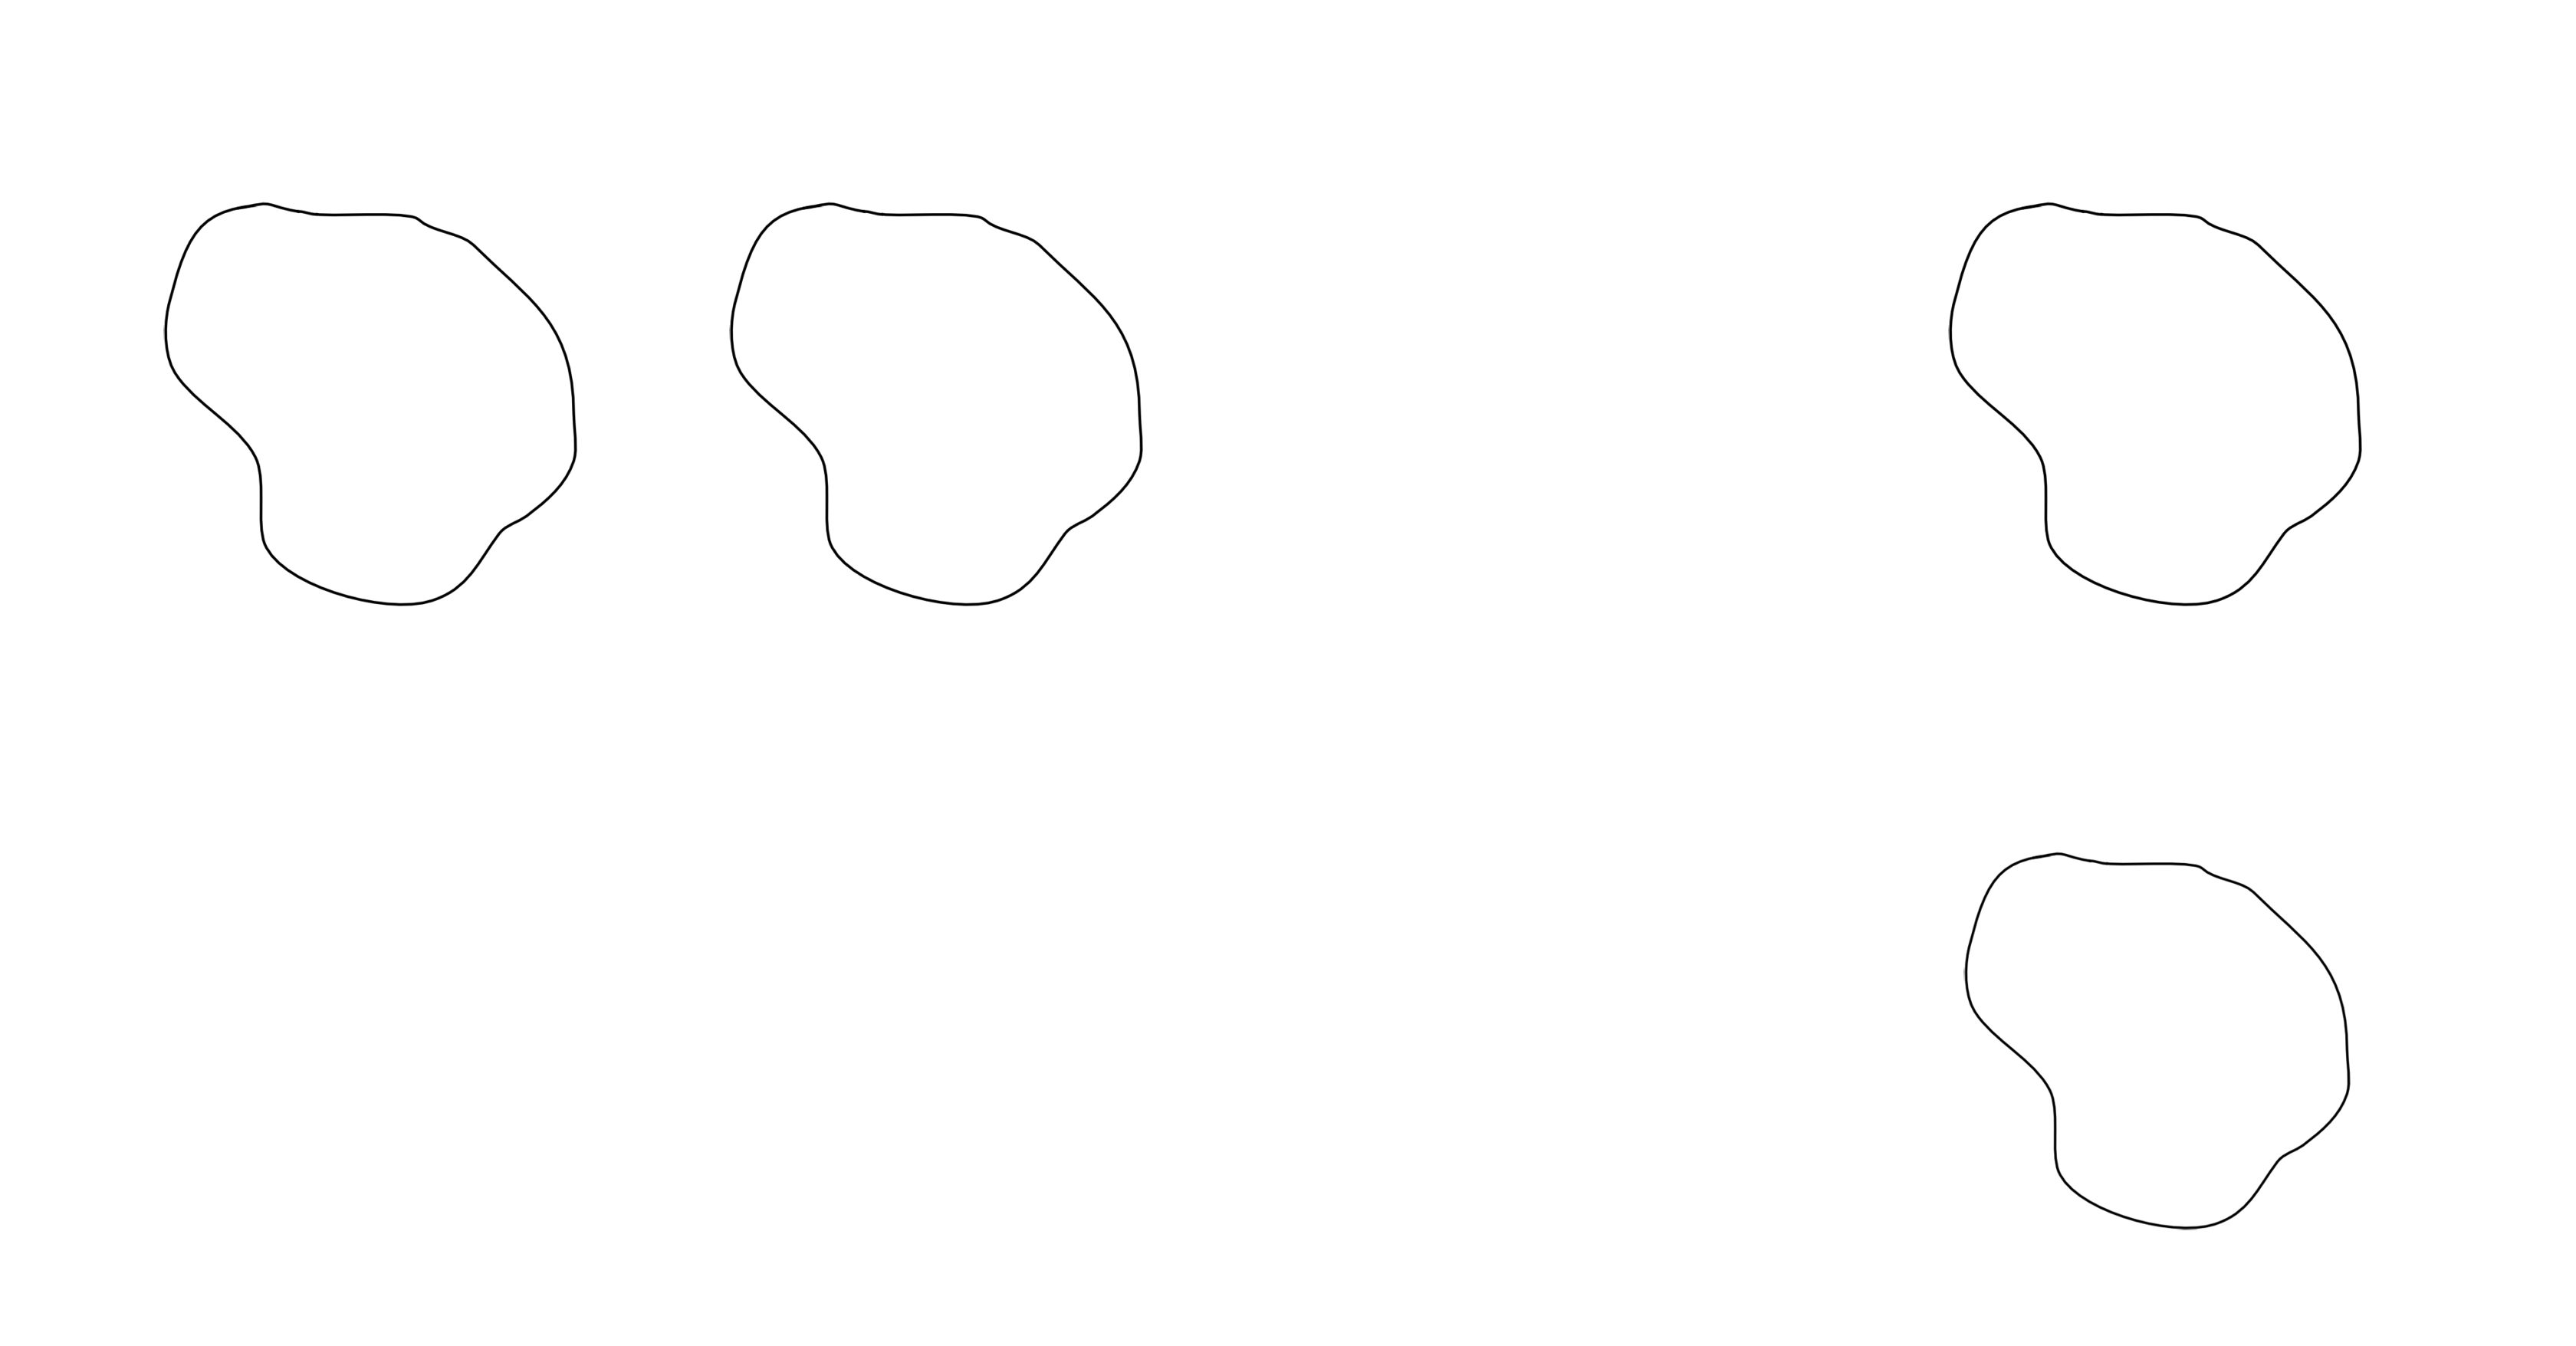
\includegraphics[width=0.95\textwidth]{figuras/ch_shift/shift-sequence.png}};
    \node at (2.3,5.8) {\large$D$};
    \node at (5.8,5.8) {\large$L^1(D)$};
    \node at (13.25,5.8) {\large$L^r(D)$};
    \node at (13.1,1.9) {\large$H$};
    \node at (9.52,5.8) {\Large$\cdots$};
    \draw[->](11.9,2.1) to [bend left,looseness=1.2] node [left]{Coloração} (11.9,5.6);
    \draw[->](5.3,7) to [bend right,looseness=1] node [above]{Lema} (2.8,7);
    \draw[->](8.8,7) to [bend right,looseness=1] node [above]{Lema} (6.3,7);
    \draw[->](12.75,7) to [bend right,looseness=1] node [above]{Lema} (10.25,7);
\end{tikzpicture}
\caption{A coloração de $H$ corresponde a uma $t$-coloração de $L^r(D)$ sem $K_{d,d}$ monocromático, e por meio de aplicações sucessivas do Lema, obtemos uma $t'$-coloração de $D$ sem $K_{t',t'}$ monocromático.}
\label{fig:shiftsequence}
\end{figure}

Mas $L^0(D) = D$, e note que todo conjunto de $2d'$ vértices de $D$ é um $K_{d',d'}$, então concluímos que existe uma $t'$ coloração de $D$ tal que nenhuma cor ocorre $2d'$ vezes, uma contradição pois se $n \geq t'(2d'-1)+1$, pelo princípio da casa dos pombos, alguma cor ocorre pelo menos $2d'$ vezes.

Portanto o número cromático de $H$ não é limitado por constante.
\end{proof}

\section{Consideração Final}

A demonstração anterior faz uso do fato que a família dos \textit{shift graphs} de ordem $r$ são grafos linha direcionados da família dos \textit{shift graphs} de ordem $r-1$. No caso de grafos linha não direcionados, podemos mostrar de forma geral que se uma família respeita a conjectura de Erd\H{o}s e Hajnal, então a família dos grafos linha também respeita a conjectura de Erd\H{o}s e Hajnal.

\begin{fato}\label{shiftconsfinal1}
Seja $\mathcal{L}$ uma família de grafos que respeita a conjectura de Erd\H{o}s e Hajnal. Então a família de grafos $L(\mathcal{L}) := \{L(G) : G\in\mathcal{L}\}$ respeita a conjectura de Erd\H{o}s e Hajnal.
\end{fato}

\begin{proof}(Fato \ref{shiftconsfinal1})
Sejam $k,g$ os parâmetros da conjectura de Erd\H{o}s e Hajnal. Seja $M$ o tamanho de um menor grafo com número cromático $k$ e cintura $g$. 

Pelo teorema de Brooks, temos que $\chi(G) \leq \Delta+1$, e como $\mathcal{L}$ respeita a conjectura de Erd\H{o}s e Hajnal, $\mathcal{L}$ tem número cromático ilimitado, e logo $\mathcal{L}$ tem grau máximo ilimitado.

Pelo teorema de Vizing, temos que $\chi'(G) = \Delta$ ou $\chi'(G) = \Delta+1$. Note que $\chi'(G) = \chi(L(G))$. E como $\mathcal{L}$ tem grau máximo ilimitado, $L(\mathcal{L})$ tem número cromático ilimitado.

Logo todo grafo $L(G)$ de $L(\mathcal{L})$ com número cromático pelo menos $M+1$ corresponde a um grafo $G$ de $\mathcal{L}$ tal que $\Delta(G) \geq M$, e um vértice de grau pelo menos $M$ em $G$ corresponde a um clique de tamanho pelo menos $M$ em $L(G)$. Portanto pela escolha de $M$, $L(G)$ contém um subgrafo com número cromático pelo menos $k$ e cintura pelo menos $g$.
\end{proof}